\documentclass[8pt,aspectratio=169]{beamer}
\usetheme{Madrid}
\usepackage{graphicx}
\usepackage{booktabs}
\usepackage{adjustbox}
\usepackage{multicol}
\usepackage{amsmath}
\usepackage{amssymb}
\usepackage{tikz}
\usepackage{hyperref}
\usepackage{algorithm}
\usepackage{algorithmic}
\usepackage{colortbl}
\usepackage{pgfplots}
\pgfplotsset{compat=1.18}

% TikZ libraries for comics, diagrams, stakeholder maps
\usetikzlibrary{arrows.meta,positioning,shapes.callouts,shapes.geometric,decorations.pathreplacing}

% Color definitions
\definecolor{mlblue}{RGB}{0,102,204}
\definecolor{mlpurple}{RGB}{51,51,178}
\definecolor{mllavender}{RGB}{173,173,224}
\definecolor{mllavender2}{RGB}{193,193,232}
\definecolor{mllavender3}{RGB}{204,204,235}
\definecolor{mllavender4}{RGB}{214,214,239}
\definecolor{mlorange}{RGB}{255, 127, 14}
\definecolor{mlgreen}{RGB}{44, 160, 44}
\definecolor{mlred}{RGB}{214, 39, 40}
\definecolor{mlgray}{RGB}{127, 127, 127}
\definecolor{lightgray}{RGB}{240, 240, 240}
\definecolor{midgray}{RGB}{180, 180, 180}

% NEW COLORS for mini-lecture
\definecolor{dfteal}{RGB}{0,128,128}
\definecolor{dfred}{RGB}{180,30,30}

% Backward compatibility
\colorlet{MLPurple}{mlpurple}
\colorlet{MLBlue}{mlblue}
\colorlet{MLOrange}{mlorange}
\colorlet{MLGreen}{mlgreen}
\colorlet{MLRed}{mlred}
\colorlet{MLLavender}{mllavender}
\colorlet{MLGray}{mlgray}

% Theme colors (exact Madrid settings)
\setbeamercolor{palette primary}{bg=mllavender3,fg=mlpurple}
\setbeamercolor{palette secondary}{bg=mllavender2,fg=mlpurple}
\setbeamercolor{palette tertiary}{bg=mllavender,fg=white}
\setbeamercolor{palette quaternary}{bg=mlpurple,fg=white}
\setbeamercolor{structure}{fg=mlpurple}
\setbeamercolor{section in toc}{fg=mlpurple}
\setbeamercolor{subsection in toc}{fg=mlblue}
\setbeamercolor{title}{fg=mlpurple}
\setbeamercolor{frametitle}{fg=mlpurple,bg=mllavender3}
\setbeamercolor{block title}{bg=mllavender2,fg=mlpurple}
\setbeamercolor{block body}{bg=mllavender4,fg=black}
\setbeamertemplate{navigation symbols}{}
\setbeamertemplate{itemize items}[circle]
\setbeamertemplate{enumerate items}[default]
\setbeamersize{text margin left=5mm,text margin right=5mm}

% Footer
\setbeamertemplate{footline}{
  \leavevmode%
  \hbox{%
    \begin{beamercolorbox}[wd=.333333\paperwidth,ht=2.25ex,dp=1ex,center]{author in head/foot}%
      \usebeamerfont{author in head/foot}Methods and Algorithms
    \end{beamercolorbox}%
    \begin{beamercolorbox}[wd=.333333\paperwidth,ht=2.25ex,dp=1ex,center]{title in head/foot}%
      \usebeamerfont{title in head/foot}MSc Data Science
    \end{beamercolorbox}%
    \begin{beamercolorbox}[wd=.333333\paperwidth,ht=2.25ex,dp=1ex,right]{date in head/foot}%
      \usebeamerfont{date in head/foot}\insertframenumber{} / \inserttotalframenumber\hspace*{2ex}
    \end{beamercolorbox}}%
  \vskip0pt%
}

\newcommand{\bottomnote}[1]{%
\vfill
\vspace{-2mm}
\textcolor{mllavender2}{\rule{\textwidth}{0.4pt}}
\vspace{1mm}
\footnotesize
\textbf{#1}
}

\newenvironment{compactlist}{%
  \begin{itemize}%
    \setlength{\itemsep}{2pt}%
    \setlength{\parskip}{0pt}%
    \setlength{\parsep}{0pt}%
}{%
  \end{itemize}%
}

\newcommand{\highlight}[1]{\textcolor{mlorange}{\textbf{#1}}}
\newcommand{\mathbold}[1]{\boldsymbol{#1}}

% ============================================================
\title[ML Paradigms Mini-Lecture]{Supervised \& Unsupervised Learning}
\subtitle{Mini-Lecture: Two Paradigms of Machine Learning}
\author{Methods and Algorithms}
\institute{MSc Data Science}
\date{}

\begin{document}

% ----------------------------------------------------------
% Slide 1: Title
% ----------------------------------------------------------
\begin{frame}[plain]
\vfill
\titlepage
\vfill
\end{frame}

% ----------------------------------------------------------
% Slide 2: XKCD Opening
% ----------------------------------------------------------
\begin{frame}{When Is a Task ``Easy''?}
\centering
\includegraphics[height=0.65\textheight]{images/1425_tasks.png}

\bottomnote{XKCD \#1425 by Randall Munroe (CC BY-NC 2.5)}
\end{frame}

% ----------------------------------------------------------
% Slide 3: What Is Machine Learning?
% ----------------------------------------------------------
\begin{frame}{What Is Machine Learning?}
\begin{columns}[T]
\begin{column}{0.55\textwidth}
\begin{compactlist}
\item Learning patterns \highlight{from data}, not from explicit programming
\item Three paradigms: \highlight{supervised}, \highlight{unsupervised}, reinforcement
\item This course: supervised (L01--L04), unsupervised (L03, L05)
\item Finance: predict defaults \emph{vs.}\ segment customers
\end{compactlist}
\end{column}
\begin{column}{0.42\textwidth}
\centering
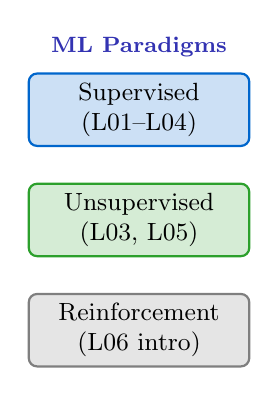
\begin{tikzpicture}[
  box/.style={draw,rounded corners=3pt,minimum width=2.8cm,
              minimum height=0.9cm,font=\small,align=center,thick},
  >=Stealth
]
  \node[box,fill=mlblue!20,draw=mlblue] (sup) at (0,2)   {Supervised\\(L01--L04)};
  \node[box,fill=mlgreen!20,draw=mlgreen] (uns) at (0,0.6) {Unsupervised\\(L03, L05)};
  \node[box,fill=mlgray!20,draw=mlgray]  (rl) at (0,-0.8) {Reinforcement\\(L06 intro)};
  \node[font=\footnotesize\bfseries,mlpurple] at (0,2.8) {ML Paradigms};
\end{tikzpicture}
\end{column}
\end{columns}

\bottomnote{Knowing which paradigm a problem belongs to is the first step in choosing an algorithm.}
\end{frame}

% ----------------------------------------------------------
% Slide 4: Supervised Learning
% ----------------------------------------------------------
\begin{frame}{Supervised Learning: Learn from Labels}
\begin{compactlist}
\item Training data consists of \highlight{$(X, y)$ pairs} --- features and a known target
\item Goal: learn a function $f: X \to y$ that \highlight{generalizes} to unseen data
\item \highlight{Regression}: $y$ is continuous (stock return, house price)
\item \highlight{Classification}: $y$ is discrete (default/no-default, sector label)
\end{compactlist}

\vspace{3mm}
\begin{block}{Core Equation}
\[
\hat{y} = f(\mathbf{x};\,\boldsymbol{\theta}) + \varepsilon
\qquad\text{where } \boldsymbol{\theta} \text{ is learned from data}
\]
\end{block}

\bottomnote{``Supervised'' = the labels $y$ supervise (guide) the learning process.}
\end{frame}

% ----------------------------------------------------------
% Slide 5: The ML Workflow
% ----------------------------------------------------------
\begin{frame}{The ML Workflow: Train / Validate / Test}
\begin{columns}[T]
\begin{column}{0.55\textwidth}
\begin{compactlist}
\item Split data: \highlight{Train 70\%} / Validation 15\% / \highlight{Test 15\%}
\item Train = fit model parameters; Validate = tune hyperparameters; Test = final evaluation
\item \highlight{Never} use test data during training --- this is \emph{data leakage}
\end{compactlist}

\vspace{2mm}
\begin{block}{Golden Rule}
The test set is opened exactly \textbf{once} --- at the very end.
\end{block}
\end{column}
\begin{column}{0.42\textwidth}
\centering
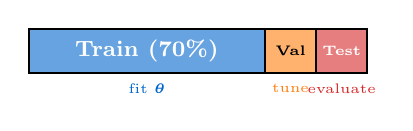
\begin{tikzpicture}[yscale=0.8]
  % bar
  \fill[mlblue!60] (0,0) rectangle (3.0,0.7);
  \fill[mlorange!60] (3.0,0) rectangle (3.65,0.7);
  \fill[mlred!60] (3.65,0) rectangle (4.3,0.7);
  % borders
  \draw[thick] (0,0) rectangle (4.3,0.7);
  \draw[thick] (3.0,0) -- (3.0,0.7);
  \draw[thick] (3.65,0) -- (3.65,0.7);
  % labels
  \node[font=\footnotesize\bfseries,white] at (1.5,0.35) {Train (70\%)};
  \node[font=\tiny\bfseries] at (3.325,0.35) {Val};
  \node[font=\tiny\bfseries,white] at (3.975,0.35) {Test};
  % percentages below
  \node[font=\tiny,mlblue] at (1.5,-0.25) {fit $\boldsymbol{\theta}$};
  \node[font=\tiny,mlorange] at (3.325,-0.25) {tune};
  \node[font=\tiny,mlred] at (3.975,-0.25) {evaluate};
\end{tikzpicture}
\end{column}
\end{columns}

\bottomnote{Data leakage is the most common source of over-optimistic results in finance ML papers.}
\end{frame}

% ----------------------------------------------------------
% Slide 6: Bias-Variance Trade-off
% ----------------------------------------------------------
\begin{frame}{Bias--Variance Trade-off}
\begin{columns}[T]
\begin{column}{0.55\textwidth}
\begin{compactlist}
\item \highlight{Underfitting} (high bias): model too simple, misses patterns
\item \highlight{Overfitting} (high variance): model memorizes noise, fails on new data
\item The \highlight{sweet spot} minimizes total error $= \text{Bias}^2 + \text{Variance}$
\item Stock prediction: fitting 50 parameters to 60 data points $\Rightarrow$ overfitting
\end{compactlist}
\end{column}
\begin{column}{0.42\textwidth}
\centering
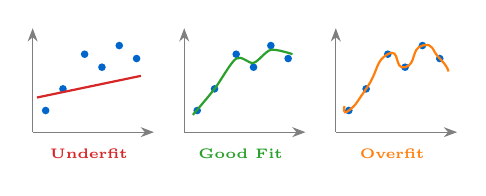
\begin{tikzpicture}[scale=0.55, >=Stealth]
  % --- Underfit ---
  \begin{scope}[shift={(0,0)}]
    \draw[->,mlgray] (0,0)--(2.8,0);
    \draw[->,mlgray] (0,0)--(0,2.4);
    \foreach \x/\y in {0.3/0.5, 0.7/1.0, 1.2/1.8, 1.6/1.5, 2.0/2.0, 2.4/1.7}
      \fill[mlblue] (\x,\y) circle(2.5pt);
    \draw[mlred,thick] (0.1,0.8) -- (2.5,1.3);
    \node[font=\tiny\bfseries,mlred] at (1.3,-0.5) {Underfit};
  \end{scope}
  % --- Good fit ---
  \begin{scope}[shift={(3.5,0)}]
    \draw[->,mlgray] (0,0)--(2.8,0);
    \draw[->,mlgray] (0,0)--(0,2.4);
    \foreach \x/\y in {0.3/0.5, 0.7/1.0, 1.2/1.8, 1.6/1.5, 2.0/2.0, 2.4/1.7}
      \fill[mlblue] (\x,\y) circle(2.5pt);
    \draw[mlgreen,thick] plot[smooth] coordinates
      {(0.2,0.4)(0.7,1.0)(1.2,1.7)(1.6,1.6)(2.0,1.9)(2.5,1.8)};
    \node[font=\tiny\bfseries,mlgreen] at (1.3,-0.5) {Good Fit};
  \end{scope}
  % --- Overfit ---
  \begin{scope}[shift={(7,0)}]
    \draw[->,mlgray] (0,0)--(2.8,0);
    \draw[->,mlgray] (0,0)--(0,2.4);
    \foreach \x/\y in {0.3/0.5, 0.7/1.0, 1.2/1.8, 1.6/1.5, 2.0/2.0, 2.4/1.7}
      \fill[mlblue] (\x,\y) circle(2.5pt);
    \draw[mlorange,thick] plot[smooth,tension=1.2] coordinates
      {(0.2,0.6)(0.3,0.5)(0.7,1.0)(1.2,1.8)(1.6,1.5)(2.0,2.0)(2.4,1.7)(2.6,1.4)};
    \node[font=\tiny\bfseries,mlorange] at (1.3,-0.5) {Overfit};
  \end{scope}
\end{tikzpicture}
\end{column}
\end{columns}

\bottomnote{Every model selection decision in this course is a bias--variance trade-off in disguise.}
\end{frame}

% ----------------------------------------------------------
% Slide 7: Unsupervised Learning
% ----------------------------------------------------------
\begin{frame}{Unsupervised Learning: Find Hidden Structure}
\begin{compactlist}
\item No labels --- only feature matrix $\mathbf{X}$; the algorithm discovers \highlight{structure}
\item \highlight{Clustering}: group similar observations (K-Means, hierarchical)
\item \highlight{Dimensionality reduction}: compress $p$ features to $k \ll p$ (PCA, t-SNE)
\item Finance applications: segment retail customers, reduce 50 stock returns to 3 latent factors
\end{compactlist}

\vspace{3mm}
\begin{block}{Key Difference from Supervised}
No ``right answer'' to evaluate against --- success is measured by \emph{coherence}
(inertia, silhouette score) not prediction accuracy.
\end{block}

\bottomnote{Unsupervised learning often serves as a preprocessing step before supervised models.}
\end{frame}

% ----------------------------------------------------------
% Slide 8: Key Terminology
% ----------------------------------------------------------
\begin{frame}{Key Terminology}
\centering
\vspace{2mm}
\begin{tabular}{@{}p{3.2cm}p{9cm}@{}}
\toprule
\textbf{Term} & \textbf{Definition} \\
\midrule
\highlight{Features} ($\mathbf{X}$)     & Input variables (predictors, covariates, independent variables) \\[2pt]
\highlight{Target} ($y$)                 & Output variable to predict (response, dependent variable) \\[2pt]
\highlight{Hyperparameter}               & Setting chosen \emph{before} training (e.g.\ learning rate, $K$ in KNN) \\[2pt]
\highlight{Cross-validation}             & Rotate train/val split $k$ times for robust performance estimate \\[2pt]
\highlight{Metric}                       & Quantitative measure of model quality (MSE, accuracy, AUC) \\
\bottomrule
\end{tabular}

\bottomnote{These five terms appear in every lecture --- make sure you can define each from memory.}
\end{frame}

% ----------------------------------------------------------
% Slide 9: Finance Applications
% ----------------------------------------------------------
\begin{frame}{Finance: Supervised vs.\ Unsupervised}
\begin{columns}[T]
\begin{column}{0.47\textwidth}
\centering
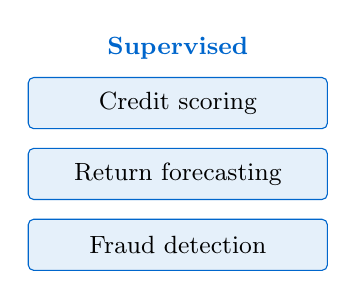
\begin{tikzpicture}[
  every node/.style={font=\small},
  box/.style={draw=mlblue,rounded corners=2pt,fill=mlblue!10,
              minimum width=3.8cm,minimum height=0.65cm,align=center}
]
  \node[font=\small\bfseries,mlblue] at (0,3.0) {Supervised};
  \node[box] at (0,2.3) {Credit scoring};
  \node[box] at (0,1.4) {Return forecasting};
  \node[box] at (0,0.5) {Fraud detection};
\end{tikzpicture}
\end{column}
\begin{column}{0.47\textwidth}
\centering
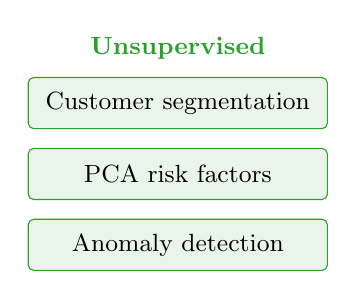
\begin{tikzpicture}[
  every node/.style={font=\small},
  box/.style={draw=mlgreen,rounded corners=2pt,fill=mlgreen!10,
              minimum width=3.8cm,minimum height=0.65cm,align=center}
]
  \node[font=\small\bfseries,mlgreen] at (0,3.0) {Unsupervised};
  \node[box] at (0,2.3) {Customer segmentation};
  \node[box] at (0,1.4) {PCA risk factors};
  \node[box] at (0,0.5) {Anomaly detection};
\end{tikzpicture}
\end{column}
\end{columns}

\vspace{4mm}
\begin{block}{In Practice}
Most production systems \highlight{combine both}: cluster customers (unsupervised), then build a classifier per segment (supervised).
\end{block}

\bottomnote{Real-world ML pipelines rarely use a single paradigm --- hybrid approaches dominate.}
\end{frame}

% ----------------------------------------------------------
% Slide 10: Summary
% ----------------------------------------------------------
\begin{frame}{Summary: Two Paradigms}
\begin{enumerate}
\setlength{\itemsep}{6pt}
\item \highlight{Supervised learning} requires labeled data $(X,y)$ and predicts outcomes
\item \highlight{Unsupervised learning} finds structure in unlabeled data $X$
\item The ML workflow (\highlight{train / validate / test}) prevents overfitting and data leakage
\item Finance uses \highlight{both paradigms}: predict defaults, segment customers, reduce dimensions
\end{enumerate}

\vspace{4mm}
\begin{block}{Coming Up}
P03: Classification \& Data Decomposition --- sorting, grouping, and compressing data.
\end{block}

\bottomnote{Every algorithm in L01--L06 falls into one of these two paradigms --- always ask ``supervised or unsupervised?''}
\end{frame}

\end{document}
